%\chapwithtoc{Přílohy}
\appendix

\chapter{Obsah přiloženého CD}

Součástí práce je kompaktní disk s následujícím obsahem:

\begin{itemize}
\item soubor \verb|readme.txt| popisující strukturu média a poskytující základní informace o práci
\item kompilovatelný zdrojový kód práce pro \LaTeX, včetně vygenerovaného PDF
\end{itemize}

\setlength{\DTbaselineskip}{4mm}
\DTsetlength{3mm}{8mm}{1mm}{0.1mm}{0.5mm}
\dirtree{%
.1 thesis/.
.2 img/.
.3 asr\_process.png.
.3 competitivity.jpg.
.3 duolingo.png.
.3 esp.png.
.3 game.jpg.
.3 logo.png.
.3 recaptcha.png.
.3 sprite.png.
.3 title\_screen.jpg.
.3 title\_stretch.jpg.
.3 trogasr.png.
.2 snip/.
.3 app.txt.
.3 cloudasr.txt.
.3 cloudasr\_final.txt.
.3 comp.txt.
.3 curry.txt.
.3 flask.txt.
.3 flask\_assets.txt.
.3 locale\_import.txt.
.3 locale\_letter.txt.
.3 locale\_options.txt.
.3 locale\_style.txt.
.3 responsive.txt.
.3 template.txt.
.2 0\_intro.tex.
.2 1\_ASR.tex.
.2 2\_e-learning.tex.
.2 3\_technologies.tex.
.2 4\_solution.tex.
.2 5\_realization.tex.
.2 6\_conclusion.tex.
.2 7\_literature.tex.
.2 8\_appendices.tex.
.2 make.bat.
.2 thesis.pdf.
.2 thesis.tex.
}

\newpage
\begin{itemize}
\item zdrojový kód a data aplikace \verb|trogASR|
\end{itemize}
\vspace{1.3mm}
\setlength{\DTbaselineskip}{3.89mm}
\DTsetlength{3mm}{8mm}{1mm}{0.1mm}{0.5mm}
\dirtree{%
.1 trogASR/.
.2 db/.
.3 cs-en.csv.
.3 en-cs.csv.
.3 import\_dict.py.
.3 schema.sql.
.3 trogasr.db.
.2 static/.
.3 css/.
.4 font.css.
.4 style.css.
.3 img/.
.4 font/.
.5 A.png.
.5 ....
.5 Z.png.
.4 ico/.
.5 cs.png.
.5 en.png.
.4 arrow-around.png.
.4 arrow-down.png.
.4 arrow-left.png.
.4 arrow-right.png.
.4 background.jpg.
.4 close-button.png.
.4 gear.gif.
.4 gears.gif.
.4 heart.png.
.4 left-banner.png.
.4 logo.png.
.3 js/.
.4 app.js.
.4 facebook.js.
.4 game.js.
.4 i18n.js.
.4 leaderboards.js.
.4 menu.js.
.4 options.js.
.4 spriteFactory.js.
.4 templates.js.
.2 templates/.
.3 components/.
.4 facebookIframe.html.
.4 facebookWidget.html.
.4 gameButton.html.
.4 leaderboardsRow.html.
.4 letter.html.
.4 localeSelectorItem.html.
.4 menuItem.html.
.4 optionsItem.html.
.4 userInfoItem.html.
.4 word.html.
.3 index.html.
.2 \_\_init\_\_.py.
.2 assets.py.
.2 configuration.py.
.2 controller.py.
.2 dao.py.
.2 LICENSE.
.2 README.md.
}

\chapter{Programátorská dokumentace}

Tato příloha popisuje v bodech konfiguraci aplikace a facebookového API, její možnou lokální instalaci a spuštění a ilustrační nasazení do jednoho z volně dostupných hostingů.

Pro detailnější popis řešených problémů a návrhu aplikace slouží kapitola \ref{chap:solution}.

\section{Konfigurace}

Pro správné fungování aplikace je nejprve nutno pozměnit nastavení v souboru \verb|configuration.py| podle požadavků. Důležité je dbát na správné nastavení cest k databázovému schématu a k \verb|.db| souboru.

Pro vývoj a úpravy je taktéž doporučeno nastavit konfiguraci {\sl DEBUG} a \mbox{{\sl ASSETS\_DEBUG}} na {\sl True}, čímž bude zajištěno dotahování neminifikovaných a nesloučených statických zdrojů a přístup k serverovému {\sl debuggeru}. Pro ostré nasazení je však doporučeno nastavit zde {\sl False}.

\subsection{Facebook API}

Pro nastavení facebookové integrace je nutné následující:

\begin{itemize}
\item přihlásit se na \url{https://developers.facebook.com/}
\item v sekci \verb|My Apps| založit novou aplikaci, zvolit \uv{WWW stránka} jako platformu
\item nechat si vygenerovat nové \verb|appID| a zanést jej do \verb|configuration.py|
\item pod záložkou \verb|Settings| nastavit jméno aplikace, domény a kontaktní e-mail
\item tamtéž vyplnit URL, kde aplikace poběží, a zanést jej taktéž do konfigurace aplikace (proměnná {\sl host})
\item v sekci \verb|Status & Review| aplikaci zveřejnit
\end{itemize}

\section{Instalace}

Pro zprovoznění aplikace \verb|trogASR| lokálně je potřeba následující:

\begin{itemize}
\item nainstalované prostředí \verb|Python| \\ \url{https://www.python.org/about/gettingstarted/}
\item nainstalovaný {\sl microframework} \verb|Flask| \\ \url{http://flask.pocoo.org/docs/0.10/installation/}
\item nainstalovaný balíček \verb|Flask-Assets| \\ \url{http://flask-assets.readthedocs.org/en/latest/}
\item spustit aplikaci \\ \verb|>python __init__.py|
\end{itemize}

\section{Nasazení}

Pro nasazení nastavené aplikace \verb|trogASR| není pak potřeba nic speciálního. Uživatel může aplikaci nasadit tak, jak je běžně zvyklý podobné aplikace nasazovat.

Pro ilustraci je zde zmíněn postup nasazení na volný hosting {\sl OpenShift}\footnote{\url{https://openshift.redhat.com}}, pročež je potřeba:

\begin{itemize}
\item zdarma vytvořit uživatelský účet \\ \url{https://www.openshift.com/}
\item stáhnout a nainstalovat klientské nástroje (\verb|rhc|) \\ \url{https://developers.openshift.com/en/managing-client-tools.html}
\item projít konfigurací nástrojů \\ \verb|>rhc setup|
\item vytvořit novou aplikaci\\ \verb|>rhc app create trogASR python-3.3|
\item lokálně klonovat \verb|git| repositář, jenž byl automaticky vytvořen --- {\sl SSH URL} je přístupné v popisu aplikace po přihlášení do {\sl OpenShift} účtu
\\ \verb|>git clone <git_url> <directory_to_create>|
\item do vzniklé složky nahrát kód aplikace, pozměnit \verb|configuration.py| --- do třídy \verb|app_config| přidat klíče
	\begin{verbatim}
	# configuration.py
	PROPAGATE_EXCEPTIONS = True
	IP = os.environ.get('OPENSHIFT_PYTHON_IP')
	PORT = int(os.environ.get('OPENSHIFT_PYTHON_PORT'))
	\end{verbatim}
\item vytvořit soubor \verb|setup.py| s nastavením popisků a balíčků
	\begin{verbatim}
	# setup.py
	from setuptools import setup, find_packages

	setup(name='trogASR',
	  version='1.0',
	  description='trogASR',
	  author='Jan Milota',
	  author_email='janek.milota@gmail.com',
	  packages=find_packages(),
	  install_requires=['Flask>=0.10.1','Flask-Assets>=0.10'])
	\end{verbatim}
\item vytvořit soubor \verb|app.py| s nastavením virtuálního prostředí a \verb|WSGI| modulu
	\begin{verbatim}
	# app.py
	import imp
	import os
	import sys
	
	try:
	  virtenv = os.path.join(
	    os.environ.get('OPENSHIFT_PYTHON_DIR','.'), 'virtenv')
	  python_version = "python" + str(sys.version_info[0])
	    + "." + str(sys.version_info[1]) 
	  os.environ['PYTHON_EGG_CACHE'] = os.path.join(
	    virtenv, 'lib', python_version, 'site-packages')
	  virtualenv = os.path.join(virtenv, 'bin','activate_this.py')
	  exec(open(virtualenv).read(), dict(__file__=virtualenv))
	except IOError:
	  pass
	  
	if __name__ == '__main__':
	  application = imp.load_source('app', '__init__.py')
	  port = application.app.config['PORT']
	  ip = application.app.config['IP']
	  from flask import Flask
	  server = Flask(__name__)
	  server.wsgi_app = application.app
	  server.run(host=ip, port=port)
	\end{verbatim}
\newpage
\item propagovat změny do \verb|git| repositáře, po čemž se automaticky provede start aplikace
	\begin{verbatim}
	>git add -A
	>git commit -m "code added!"
	>git push
	\end{verbatim}
\end{itemize}

\chapter{Uživatelská dokumentace}
\label{appendix:user_doc}

Tato příloha popisuje samotnou hru \verb|trogASR| z pohledu hráče (uživatele) hry. Zabývá se lehkým popisem už tak dostatečně intuitivní hry, kde vypichuje jednotlivé uživatelské možnosti a zmiňuje, co znamenají. Na konci přílohy čtenář nalezne základní postup {\sl troubleshootingu} (odstraňování problémů).

\section{Popis hry}

Hra \verb|trogASR| je ve svém jádře velice jednoduchá. Po rychlém a intuitivním nastavení lze vplout přímo do akce. Doporučeným postupem je hned po načtení stisknout tlačítko \uv{Log In} a přihlásit se, aby se hráč mohl umisťovat v žebříčcích. Samosebou, stisk ostatních tlačítek v pravém horním rohu je též žádoucí.

Stisk tlačítek v rohu levém horním ovládá jazykové nastavení zobrazení hry. Tento jazyk je pouze použit pro zobrazení a nemá nic společného s jazyky herními.

Aplikace si po načtení žádá přístup k volnému vstupnímu zvukovému zařízení. Tento přístup je nutno jí poskytnout, chce-li hráč hrát. Většina prohlížečů při získání tohoto přístupu ztlumí ostatní běžící aplikace. Po konci herního sezení lze pro návrat do původního stavu buďto přístup aplikaci odepřít, nebo záložku se hrou zavřít.

\begin{figure}[h]
	\centering
	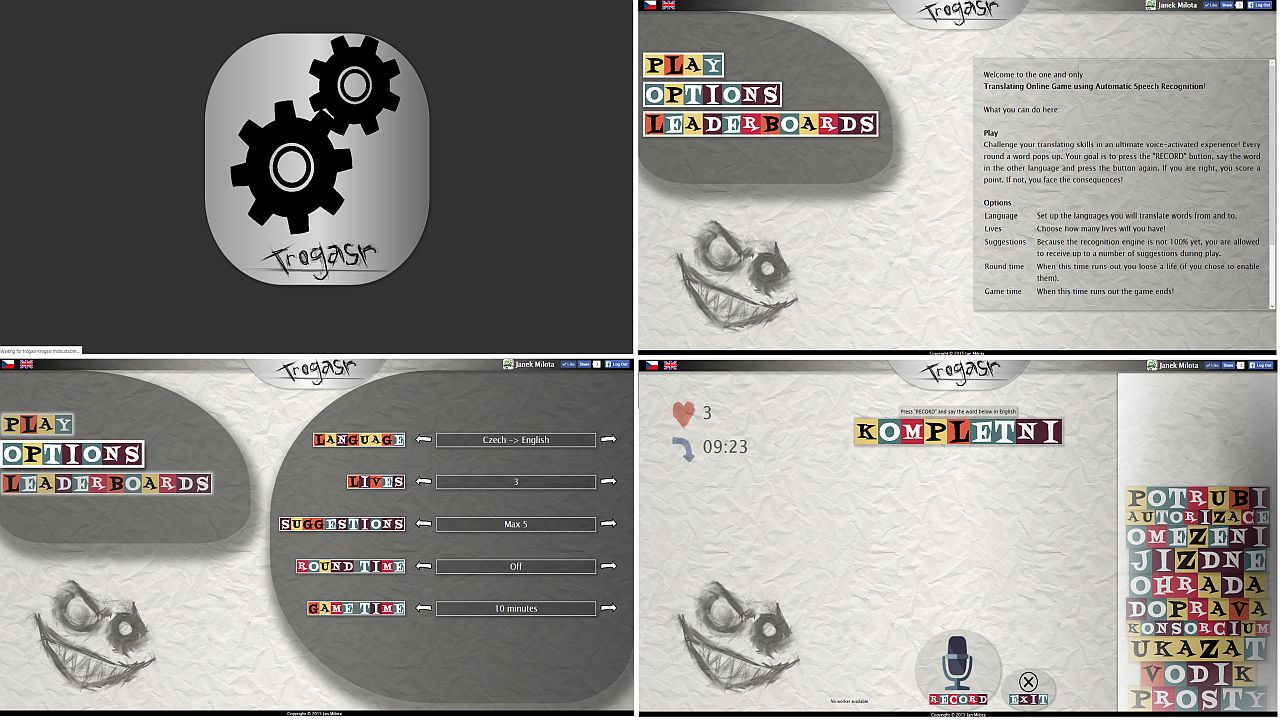
\includegraphics[width=140mm,height=80mm]{img/trogasr.jpg}
	\caption{Ukázka některých herních obrazovek.}
	\label{fig:trogasr}
\end{figure}

\subsection{Play - Hrát}

Každé kolo sestává z těchto kroků:

\begin{itemize}
\item vyskočení slova ve zdrojovém jazyce
\item stisk tlačítka nahrávání
\item vyřčení slova v jazyce cílovém
\item puštění stisknutého tlačítka nahrávání
\end{itemize}

Pokud hráč vysloví slovo správně a rozpoznávač řeči vrátí řetězec, který se vyskytuje v alespoň jednom z významů slova, kolo skončí úspěchem --- současné slovo skočí do zásobníku správně přeložených slov.

Pokud se slovo rovnou nerozpozná a je nastavena možnost nápovědy, pak se hráči zobrazí maximálně nastavený počet nápověd, mezi kterými je zaručeně alespoň jeden ze správných překladů slova. Při kliku na správný překlad kolo skončí úspěchem. Při špatné volbě kolo skončí neúspěchem a ubude hráči život (pokud jsou tyto nastaveny).

V případě, že hráč nastavil nějaký čas kola, po vypršení tohoto času kolo rovnou skončí neúspěchem.

Je-li nastaven čas na hru, po jeho vypršení skončí celá hra a vypíše se dosažený počet bodů. Dojdou-li hráči životy, stane se to samé.

Hru lze kdykoli násilně ukončit tlačítkem ukončovacím.

\subsection{Options - Nastavení}

Nastavení hry \verb|trogASR| je velice snadné a pochopí jej opravdu každý.

Lze nastavit tyto volby:

\begin{itemize}
\item dvojice zdrojový a cílový jazyk
\item počet životů --- možno úplně vypnout
\item maximální počet nápověd --- možno též úplně vypnout
\item čas na kolo
\item čas na hru
\end{itemize}

V základu jsou přednastaveny volby pro většinu hráčů, příchozích poprvé, dostatečně pohodlné.

\subsection{Leaderboards - Žebříčky}

V sekci žebříčků je ukázán seznam jmen hráčů a jimi dosažené počty bodů, seřazené od nejvyššího po nejnižší. Těmito lze volně brouzdat a závidět těm nejlepším.

Pro umístění v žebříčcích musí být hráč přihlášen a musí dokončit hru s alespoň jedním získaným bodem.

\section{Troubleshooting}

V případě, že hráči hra z nějakého důvodu nefunguje, nechť vyzkouší v tomto pořadí:

\begin{itemize}
\item ověřit připojení k aplikaci
\item zavřít a znovu otevřít prohlížeč
\item nainstalovat aktualizace prohlížeče
\item vyzkoušet jiný podporovaný prohlížeč
\item restartovat operační systém
\item nainstalovat systémové updaty
\item updatovat ovladače zvukových zařízení
\item kontaktovat správce své sítě
\item kontaktovat autora této práce
\end{itemize}